\chapter{Implementation Notes}

\cvmfs\ has a modular structure and relies on several open source libraries.
Figure~\ref{fig:cvmfsblocks} shows the internal building blocks of \cvmfs.
Most of these libraries are shipped with the \cvmfs\ sources and are linked statically in order to facilitate debugging and to keep the system dependencies minimal.

\begin{figure}
	\begin{center}
		%\documentclass[a4paper, 11pt]{article}

%\usepackage{tikz,ifthen}
%\usetikzlibrary{shapes,matrix,shadows,fit,backgrounds}

%\begin{document}
\begin{tikzpicture}
\edef\blockwidth{7em} 
\edef\blockheight{2.5em}
\scope[ 
      block/.style={
         anchor=south west,
         rectangle,
         very thick,
         drop shadow,
         rounded corners=3mm,
         minimum width=\blockwidth,
         minimum height=\blockheight},   
      buildingblock/.style={
         block,
         draw=red!50!black!50,
         top color=white,
         bottom color=red!50!black!20},
      module/.style={
         block,
         draw=green!50!black!50,
         top color=white,
         bottom color=green!50!black!20},
      fuse/.style={
         block,
         draw=blue!50!black!50,
         top color=white,
         bottom color=blue!50!black!20},
      blocklabel/.style={
         anchor=north west,
         inner ysep=-0.5ex,
         font=\large\sf},
      every fit/.style={
         rectangle,
         very thick,
         draw=gray},
      font={\small\sf}
   ]
   
   \edef\spacesep{2ex}
   \edef\numofelemsperline{3}

   % Bulding Blocks
   \edef\numofelems{8} 
   \pgfmathparse{floor(\numofelems/\numofelemsperline)*\numofelemsperline}\edef\fitsuntil{\pgfmathresult}
   \foreach \i / \name in {0 / SHA1, 1 / MD5, 2 / zlib, 3 / SQLite, 4 / libcurl, 5 / libcrypto, 6 / Fuse, 7 / redirfs}
   {
      \ifthenelse{\i<\fitsuntil}{\edef\offset{0}}{
         \pgfmathparse{((\numofelemsperline-mod(\numofelems,\numofelemsperline))/2)*(\blockwidth+\spacesep)}\edef\offset{\pgfmathresult}}
      \pgfmathparse{\offset + mod(\i,\numofelemsperline)*(\blockwidth+\spacesep)}\edef\blockx{\pgfmathresult}
      \pgfmathparse{floor(\i/\numofelemsperline) * (\blockheight+\spacesep)}\edef\blocky{\pgfmathresult}
      \coordinate (blockxy) at (\blockx pt, \blocky pt);
      \node [buildingblock] at (blockxy) {\name};
   }
   \pgfmathparse{\numofelemsperline*(\blockwidth+\spacesep)-\spacesep}\edef\extremx{\pgfmathresult}
   \pgfmathparse{ceil(\numofelems/\numofelemsperline)*(\blockheight+\spacesep)-\spacesep + 4ex}\edef\extremy{\pgfmathresult}
   \coordinate (extremxy) at (\extremx pt, \extremy pt);
   \node (bb bottom left) at (0,0) {};
   \node (bb top right) at (extremxy) {};
   \begin{pgfonlayer}{background}
      \node [fit=(bb bottom left) (bb top right),top color=red!50!black!20,bottom color=white] (bb box) {};
      \node [blocklabel] at (0,\extremy pt) {Building Blocks};
   \end{pgfonlayer}
   

   % Modules
   \pgfmathparse{\extremy+2*\spacesep}\edef\yoffset{\pgfmathresult}
   \edef\numofelems{5}
   \pgfmathparse{floor(\numofelems/\numofelemsperline)*\numofelemsperline}\edef\fitsuntil{\pgfmathresult}
   \foreach \i / \name in {0 / Catalog, 1 / Cache, 2 / {Quota / LRU}, 3 / Trace Capturing, 4 / {VFS Filter}}
   {
      \ifthenelse{\i<\fitsuntil}{\edef\offset{0}}{
         \pgfmathparse{((\numofelemsperline-mod(\numofelems,\numofelemsperline))/2)*(\blockwidth+\spacesep)}\edef\offset{\pgfmathresult}}
      \pgfmathparse{\offset + mod(\i,\numofelemsperline)*(\blockwidth+\spacesep)}\edef\blockx{\pgfmathresult}
      \pgfmathparse{\yoffset + floor(\i/\numofelemsperline) * (\blockheight+\spacesep)}\edef\blocky{\pgfmathresult}
      \coordinate (blockxy) at (\blockx pt, \blocky pt);
      \node [module] at (blockxy) {\name};
   }
   \pgfmathparse{\numofelemsperline*(\blockwidth+\spacesep)-\spacesep}\edef\extremx{\pgfmathresult}
   \pgfmathparse{\yoffset+ceil(\numofelems/\numofelemsperline)*(\blockheight+\spacesep)-\spacesep + 4ex}\edef\extremy{\pgfmathresult}
   \coordinate (extremxy) at (\extremx pt, \extremy pt);
   \node (mod bottom left) at (0,\yoffset pt) {};
   \node (mod top right) at (extremxy) {};
   \begin{pgfonlayer}{background}
      \node [fit=(mod bottom left) (mod top right),top color=green!50!black!20,bottom color=white] (mod box) {};
      \node [blocklabel] at (0,\extremy pt) {Components};
   \end{pgfonlayer}
   
   %fuse
   \pgfmathparse{\extremy+2*\spacesep}\edef\yoffset{\pgfmathresult}
   \edef\numofelems{2}
   \pgfmathparse{floor(\numofelems/\numofelemsperline)*\numofelemsperline}\edef\fitsuntil{\pgfmathresult}
   \foreach \i / \name in {0 / \cvmfs, 1 / cvmfs\_sync}
   {
      \ifthenelse{\i<\fitsuntil}{\edef\offset{0}}{
         \pgfmathparse{((\numofelemsperline-mod(\numofelems,\numofelemsperline))/2)*(\blockwidth+\spacesep)}\edef\offset{\pgfmathresult}}
      \pgfmathparse{\offset + mod(\i,\numofelemsperline)*(\blockwidth+\spacesep)}\edef\blockx{\pgfmathresult}
      \pgfmathparse{\yoffset + floor(\i/\numofelemsperline) * (\blockheight+\spacesep)}\edef\blocky{\pgfmathresult}
      \coordinate (blockxy) at (\blockx pt, \blocky pt);
      \node [fuse] at (blockxy) {\name};
   }
   \pgfmathparse{\numofelemsperline*(\blockwidth+\spacesep)-\spacesep}\edef\extremx{\pgfmathresult}
   \pgfmathparse{\yoffset+ceil(\numofelems/\numofelemsperline)*(\blockheight+\spacesep)-\spacesep + 4ex}\edef\extremy{\pgfmathresult}
   \coordinate (extremxy) at (\extremx pt, \extremy pt);
   \node (fuse bottom left) at (0,\yoffset pt) {};
   \node (fuse top right) at (extremxy) {};
   \begin{pgfonlayer}{background}
      \node [fit=(fuse bottom left) (fuse top right),top color=blue!50!black!20,bottom color=white] (fuse box) {};
      \node [blocklabel] at (0,\extremy pt) {User Interface};
   \end{pgfonlayer}      
\endscope
\end{tikzpicture}
%\end{document}

	\end{center}
	\caption{\cvmfs\ building blocks.}
	\label{fig:cvmfsblocks}
\end{figure}


\section{File Catalog}

A \cvmfs\ repository is defined by its \emph{file catalog}.
The file catalog is an \sqlite\footnote{\url{https://www.sqlite.org}} database~\cite{sqlite10} having a single table that lists files and directories together with its metadata.
The table layout is shown in Table~\ref{tab:catalog}.

\begin{table}
	\begin{center}
		\begin{tabular}[b]{ccc}
			\begin{tabular}{ll}
				\toprule
				\bf Field & \bf Type \\
				\midrule
				\bf Path MD5		& 128\,Bit Integer \\
				Parent Path MD5		& 128\,Bit Integer \\
				Hardlinks			& Integer \\
				SHA1 Content Hash	& 160\,Bit Integer \\
				Size 				& Integer\\
				Mode 				& Integer \\
				Last Modified 		& Timestamp \\
				Flags 				& Integer \\
				Name 				& String \\
				Symlink 			& String \\
				uid 				& Integer \\
				gid 				& Integer \\
				\bottomrule
			\end{tabular} &
			\qquad & 
			\begin{tabular}{ll}
				\toprule
				\bf Flags & \bf Meaning\\
				\midrule
				1		& Directory \\
				2		& Transition point to a nested catalog \\
				33		& Root directory of a nested catalog \\
				3		& Regular file \\
				4		& Symbolic link \\
				\bottomrule
			\end{tabular}
		\end{tabular}
	\end{center}
	\caption{Metadata information stored per directory entry.  
		The inode is dynamically issued by \cvmfs\ at runtime.}
	\label{tab:catalog}
\end{table}

In order to save space we do not store absolute paths.
Instead we store MD5~\cite{rfc1321,rfc6151} hash values of the absolute path names.
Symbolic links are kept in the catalog.
Symbolic links may contain environment variables in the form \texttt{\$(VAR\_NAME)} or \texttt{\$(VAR\_NAME:-/default/path)}  that will be dynamically resolved by \cvmfs\ on access.
Hardlinks are emulated by \cvmfs.
The hardlink count is stored in the lower 32bit of the hardlinks field, a \emph{hardlink group} is stored in the higher 32 bit.
If the hardlink group is greater than zero, all files with the same hardlink group will get the same inode issued by the \cvmfs\ Fuse client.
The emulated hardlinks work within the same directory, only.
The cryptographic content hash refers to the zlib-compressed~\cite{rfc1950} version of the file.
Flags indicate the type of an directory entry (see Table~\ref{tab:catalog}).

A file catalog contains a \emph{time to live} (TTL), stored in seconds.
The catalog TTL advises clients to check for a new version of the catalog, when expired.
Checking for a new catalog version takes place with the first file system operation on a \cvmfs\ volume after the TTL has expired.
The default TTL is 15 minutes.
If a new catalog is available, \cvmfs\ delays the loading for the period of the \cvmfs\ kernel cache life time (default: 1~minute).
During this drain-out period, the kernel caching is turned off.
The first file system operation on a \cvmfs\ volume after that additional delay will apply a new file catalog and kernel caching is turned back on.

\subsection{Content Hashes}
\cvmfs\ can use SHA-1~\cite{rfc3174} or RIPEMD-160~\cite{ripemd160} as cryptographic hash function.
The hash function can be changed on the Stratum 0 during the lifetime of repositories.
On a change, new and updated files will use the new cryptographic hash while existing files remain unchanged.
This is transparent to the clients since the hash function is stored in the flags field of file catalogs for each and every file.
The default hash function is SHA-1.
New software versions might introduce support for further cryptographic hash functions.

\subsection{Nested Catalogs}
In order to keep catalog sizes reasonable\footnote{As a rule of thumb, file catalogs up to \SI{25}{\mega\byte} (compressed) are reasonably small.}, repository subtrees may be cut and stored as separate \emph{nested catalogs}.
There is no limit on the level of nesting.
A reasonable approach is to store separate software versions as separate nested catalogs.
Figure~\ref{fig:nested} shows the simplified directory structure which we use for the ATLAS repository.
\begin{figure}
	\begin{center}
		\framebox{%\documentclass[a4paper, 11pt]{article}

%\include{jtex}
%\usepackage{tikz,ifthen}
%\usetikzlibrary{arrows,positioning,shapes,topaths,calc,fit,backgrounds,matrix,shadows}

%\begin{document}

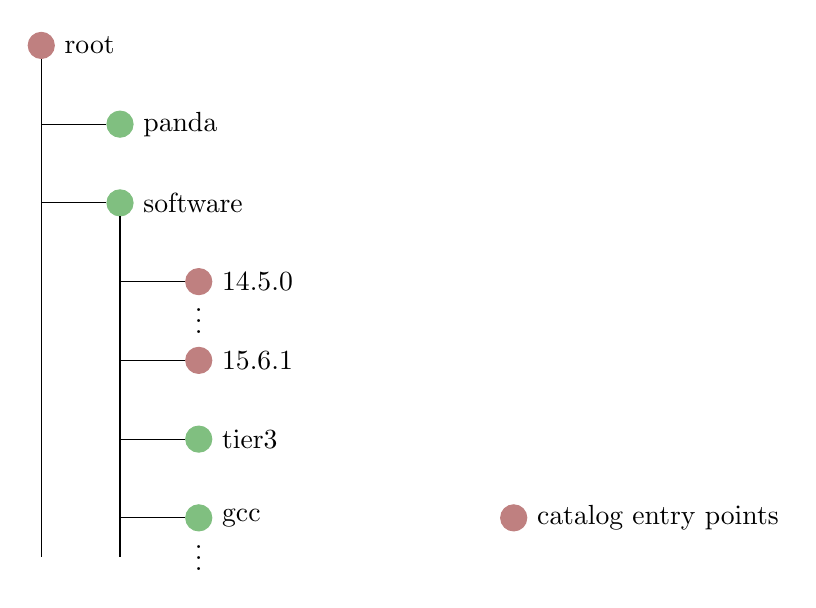
\begin{tikzpicture}
	[
		dirent/.style={
			circle,
			draw=green!50!black!50,
			fill=green!50!black!50
		}
	]
	\node[dirent,label=right:root,red!50!black!50,fill=red!50!black!50] (root) at (0,0) {};
	\node[dirent,label=right:panda] (panda) at (1, -1) {};
	\node[dirent,label=right:software] (software) at (1, -2) {};
	\node[dirent,label=right:14.5.0,red!50!black!50,fill=red!50!black!50] (1450) at (2, -3) {};
	\node[] (dots1) at (2, -3.4) {$\vdots$};
	\node[dirent,label=right:15.6.1,red!50!black!50,fill=red!50!black!50] (1561) at (2, -4) {};
	\node[dirent,label=right:tier3] (tier3) at (2, -5) {};
	\node[dirent,label=right:gcc] (gcc) at (2, -6) {};
	\node[] (dots2) at (2, -6.4) {$\vdots$};
	\node[dirent,label=right:catalog entry points,red!50!black!50,fill=red!50!black!50] (key) at (6,-6) {};
	
	%\node[dirent] (d2) at (0.4, 0.8) {};
	%\node[dirent,red!50!black!50,fill=red!50!black!50] (d21) at (0.8, 0.4) {};
	%\node[dirent] (d22) at (0.8, 0) {};
	%\node[scale=0.175] (file) at (2, 0.8) {\pdfimage{file.pdf}};
	
	\draw (root) -- (0,-1) -- (panda);
	\draw (0,-1) -- (0,-2) -- (software);
	\draw (0,-2) -- (0,-6.5);
	\draw (software) -- (1,-3) -- (1450);
	\draw (1,-3) -- (1,-4) -- (1561);
	\draw (1,-4) -- (1,-5) -- (tier3);
	\draw (1,-5) -- (1,-6) -- (gcc);
	\draw (1,-6) -- (1,-6.5);
\end{tikzpicture}
%\end{document}}
	\end{center}
	\caption{Directory structure useds for the ATLAS repository (simplified).}
	\label{fig:nested}
\end{figure}

When a subtree is moved into a nested catalog, its entry directory serves as \emph{transition point} for nested catalogs.
This directory appears as empty directory in the parent catalog with flags set to 2.
The same path appears as root-directory in the nested catalog with flags set to 33.
Because the MD5 hash values refer to full absolute paths, nested catalogs store the root path prefix.
This prefix is prepended transparently by \cvmfs.
The cryptographic hash of nested catalogs is stored in the parent catalog.
Therefore, the root catalog fully defines an entire repository.

Loading of nested catalogs happens on demand by \cvmfs\ on the first attempt to access of anything inside, \ie a user won't see the difference between a single large catalog and several nested catalogs.
While this usually avoids unnecessary catalogs to be loaded, recursive operations like \texttt{find} can easily bypass this optimization.

\subsection{Catalog Statistics}
A \cvmfs\ file catalog maintains several counters about its contents and the contents of all of its nested catalogs. 
The idea is that the catalogs know how many entries there are in their sub catalogs even without opening them.
This way, one can immediately tell how many entries, for instance, the entire ATLAS repository has. 
Some of the numbers are shown using the number of inodes in \texttt{statvfs}. 
So \texttt{df -i} shows the overall number of entries in the repository and (as number of used inodes) the number of entries of currently loaded catalogs. 
Nested catalogs create an additional entry (the transition directory is stored in both the parent and the child catalog). 
File hardlinks are still individual entries (inodes) in the cvmfs catalogs.
The following counters are maintained for both a catalog itself and for the subtree this catalog is root of:
\begin{itemize}
	\item Number of regular files
	\item Number of symbolic links
	\item Number of directories
	\item Number of nested catalogs
	\item Number of chunked files
	\item Number of individual file chunks
	\item Overall file content size
	\item File content size stored in chunked files
\end{itemize}

%\subsection{$\mu$-Catalogs}
%The $\mu$-catalogs can be constructed in addition to the normal file catalogs.
%The $\mu$-catalogs can be considered as a special case of nested catalogs, in which each directory is a nested catalog.
%Essentially they are a precalculated \texttt{ls -la} for all directories.
%They are implemented as SQlite catalogs as well having the same structure as normal catalogs.
%The SHA-1 content hashes of the $\mu$-catalogs are stored in the hash field of the directory entries in the catalog table.

\pagebreak
\section{Repository Manifest (.cvmfspublished)}
\label{sct:cvmfspublished}
Every \cvmfs\ repository contains a repository manifest file that serves as entry point into the repository's catalog structure.
The repository manifest is the first file accessed by the \cvmfs\ client at mount time and therefore must be accessible via HTTP on the repository root URL.
It is always called \textbf{.cvmfspublished} and contains fundamental repository meta data like the root catalog's cryptographic hash and the repository revision number as a key-value list.

\subsection{Internal Manifest Structure}
Below is an example of a typical manifest file.
Each line starts with a capital letter specifying the meta data field, followed by the actual data string.
The list of meta information is ended by a separator line (\texttt{-{}-}) followed by signature information further described in Section~\ref{sct:cvmfspublished:signature}.
Please refer to table~\ref{tbl:manifestfields} for detailed information about each of the meta data fields.

\begin{table}
	\begin{center}
		\begin{tabularx}{\linewidth}{lX}
			\toprule
			{\bf\centering Field} & {\bf\centering Meta Data Description} \\
			\midrule
			\texttt{C} & Cryptographic hash of the repository's current root catalog \\
			\texttt{R} & \begin{tabular}[t]{@{}l@{}}MD5 hash of the repository's root path\\(usually always \texttt{d41d8cd98f00b204e9800998ecf8427e})\end{tabular} \\
			\texttt{B} & File size of the root catalog in bytes \\
			\texttt{X} & Cryptographic hash of the signing certificate \\
			\texttt{H} & Cryptographic hash of the repository's named tag history database \\
			\texttt{T} & Unix timestamp of this particular revision \\
			\texttt{D} & Time To Live (TTL) of the root catalog \\
			\texttt{S} & Revision number of this published revision \\
			\texttt{N} & The full name of the manifested repository \\
			\texttt{L} & currently unused (reserved for micro catalogs) \\
			\bottomrule
		\end{tabularx}
	\end{center}
	\caption{Meaning of Repository Manifest Meta Data Fields}
	\label{tbl:manifestfields}
\end{table}

\begin{verbatim}
    C64551dccfbe0a48de7618dd7deb290200b474759
    B1442336
    Rd41d8cd98f00b204e9800998ecf8427e
    D900
    S42
    Nexample.cern.ch
    X731cca9476eb882f5a3f24aaa38001105a0e35eb
    T1390301299
    --
    edde5308e502dd5e8fe405c56f5700f7477dc319
    [...]
\end{verbatim}

\subsection{Repository Signature}
\label{sct:cvmfspublished:signature}
In order to provide authoritative information about a repository publisher, the repository manifest is signed by an X.509 certificate together with its private key.

\subsubsection{Signing a Repository}
It is important to note that it is sufficient to sign just the manifest file itself to gain a secure chain of the whole repository.
The manifest refers to the cryptographic content hash of the root catalog which in turn recursively references all sub-catalogs with their cryptographic content hashes.
Each catalog lists its files along with their cryptographic content hashes.
This concept is called a merkle tree and eventually provides a single hash that depends on the \textit{complete} content of the repository.

The top level hash used for the repository signature can be found in the repository manifest right below the separator line (\texttt{-{}-} / see above).
It is the cryptographic hash of the manifest's meta data lines excluding the separator line.
Following the top level hash is the actual signature produced by the X.509 certificate signing procedure in binary form.

\subsubsection{Signature Validation}
In order to validate repository manifest signatures, \cvmfs\ uses a white-list of valid publisher certificates.
The white-list contains the cryptographic fingerprints of known publisher certificates and a timestamp.
A white-list is valid for 30 days.
It is signed by a private RSA key, which we refer to as \emph{master key}.
%For the cern.ch repositories, the master key is kept offline on a secure smart card at \cern.
%So the security of the master key is ensured by 2-factor authentication (possession of the smart card and knowledge of the pin).
%The smart card is used with a smart card reader with pin pad.
%Neither the key nor the pin are ever exposed outside the scope of those secure devices.
The public RSA key that corresponds to the master key is distributed with the \texttt{cvmfs-config-$\cdots$} RPMs as well as with every instance of \cernvm.

In addition, \cvmfs\ checks certificate fingerprints against the local blacklist /etc/cvmfs/blacklist.
The blacklisted fingerprints have to be in the same format than the fingerprints on the white-list.
The blacklist has precedence over the white-list.

As crypto engine, \cvmfs\ uses \product{libcrypto} from the \product{OpenSSL} project~\cite{openssl}.
%Figure~\ref{fig:security} shows the trust chain with a signed repository.
%\begin{figure}
%	\begin{center}
%		%\documentclass[a4paper, 11pt]{article}\usepackage{tikz,ifthen}\usetikzlibrary{arrows,positioning,shapes,topaths,calc,fit,backgrounds,matrix,shadows}\begin{document}

\begin{tikzpicture}
	[block/.style={node distance=1cm,rounded corners,draw,minimum height=0.7cm,minimum width=3cm},
	 fig/.style={}]
	
	\node[fig,gray] (release manager) at (6cm,0cm) {\parbox{2cm}{\centering release\\
\includegraphics[width=1.25cm]{figures/releasemanager}\\manager}};
	\node[fig,gray,anchor=north] (whitelist) at (0cm,-2cm) {\parbox{3cm}{\centering \parbox[top][2cm][c]{2.5cm}{
\includegraphics[width=2.5cm]{figures/cernvm}}\\certificate white-list}};
	\node[fig,gray,anchor=north] (web server) at (12cm,-2cm) {\parbox{3cm}{\centering \parbox[top][2cm][c]{2.5cm}{
\includegraphics[width=1.75cm]{figures/webserver}}\\repository}};
	\node[block,green!50!black,very thick] (cvmfs) at (6cm,-9cm) {\parbox{3.5cm}{\centering{\scshape CernVM-FS +\\CernVM} public key}};
	
	\draw[->,gray,very thick] (release manager.west) -- node[gray,fill=white] {\parbox{2cm}{\centering
\includegraphics[width=1cm]{figures/fingerprint}\\ fingerprint}} (whitelist.north);
	\draw[->,gray,very thick] (release manager.east) -- node[gray,fill=white] {\parbox{2cm}{\centering
\includegraphics[width=1cm]{figures/sign-cert}\\ sign repository}} (web server.north);
	\draw[->,gray,very thick] (whitelist.east) -- node[white,fill] {\parbox{2cm}{\centering
\includegraphics[width=1cm]{figures/sign}\\ \textcolor{gray}{sign whitelist}}} ($(whitelist.east) + (8.75,0)$);
	
	\draw[->,very thick,blue!75,curve to,out=200,in=90] (web server.south west) to node[blue!75,fill=white] {\parbox{3cm}{\centering {\tikz \node[fill,draw,circle,inner sep=1pt]{\textcolor{white}1};}\\download\\signed catalog +\\signed whitelist}} (cvmfs.north);
	\node[blue!75,above left=of cvmfs,xshift=0.75cm,yshift=-0.75cm] {\parbox{3cm}{\centering {\tikz \node[fill,draw,circle,inner sep=1pt]{\textcolor{white}2};}\\verify whitelist +\\check fingerprint}};
	\draw[->,very thick,blue!75,curve to,out=270,in=45] (web server.south) to node[blue!75,below] {\parbox{2cm}{\centering {\tikz \node[fill,draw,circle,inner sep=1pt]{\textcolor{white}3};}\\download\\files}} (cvmfs.north east);
	\node[blue!75] at (6cm,-10.5cm) {\parbox{4cm}{\centering {\tikz \node[fill,draw,circle,inner sep=1pt]{\textcolor{white}4};}\\compare secure hash\\against catalog entry}};
\end{tikzpicture} 

%\end{document}

%	\end{center}
%	\caption{Trust chain with a signed repository.}
%	\label{fig:security}
%\end{figure}


%\section{Repository Layout}
%\label{sct:repository}

\pagebreak
\section{Use of HTTP}
The particular way of using the \indexed{HTTP} protocol has significant impact on the performance and usability of \cvmfs.
If possible, \cvmfs\ tries to benefit from the HTTP/1.1 features keep-alive and cache-control.
Internally, \cvmfs\ uses the \product{libcurl} library~\cite{libcurl}.

The HTTP behaviour affects a system with cold caches only.
As soon as all necessary files are cached, there is only network traffic when a catalog TTL expires.
%Usually we'll see network traffic right after booting a \cernvm\ for the first time, after switching to another experiment environment, and after a new software version has been published.

The \cvmfs\ download manager runs as a separate thread that handles download requests asynchronously in parallel.
Concurrent download requests for the same URL are collapsed into a single request.

\subsection{DoS Protection}
A subtle denial of service attack (DoS) can occur when \cvmfs\ is successfully able to download a file but fails to store it in the local cache.
This situation escalates into a DoS when the application using \cvmfs\ remains in an endless loop and tries to open a file over and over again.
Such a situation is prevented by \cvmfs\ by re-trying with an exponential backoff.
%That prevents request storms to web servers from applications trying to open a file in an endless loop.
The backoff is triggered by consequtive filaures to cache a downloaded file within 10 seconds.

\subsection{Keep-Alive}
Although the HTTP protocol overhead is small in terms of data volume, in high latency networks we suffer from the bare number of requests: Each request-response cycle has a penalty of at least the network round trip time. 
Using plain HTTP/1.0, this results in at least $3\cdot\text{round trip time}$ additional running time per file download for TCP handshake, HTTP GET, and TCP connection finalisation.
By including the \texttt{Connection:~Keep-Alive} header into HTTP requests, we advise the HTTP server end to keep the underlying TCP connection opened.
This way, overhead ideally drops to just round trip time for a single HTTP GET.
The impact of the keep-alive feature is shown in Figure~\ref{fig:keepalive}.
\begin{figure}
	\begin{center}
		\resizebox{0.5\linewidth}{!}{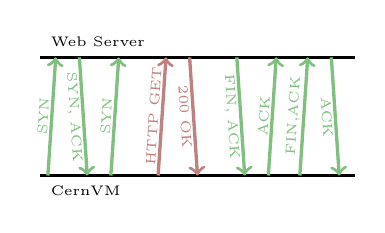
\begin{tikzpicture}
	[
		legend/.style={
			font=\tiny,
			outer sep=-2pt
		},
		legendframe/.style={
			font=\tiny
		},
		seq/.style={
			->, 
			very thick, 
			green!50!black!50	
		},
		http/.style={
			->, 
			very thick, 
			red!50!black!50	
		}
	]
	
	\draw[very thick]  (0,1.5) -- node[legendframe,above,anchor=south west] {Web Server} (0,1.5) -- (4,1.5);
	\draw[very thick]  (0,0) -- node[legendframe,below,anchor=north west] {CernVM} (0,0) -- (4,0);
	
	\draw[seq] (0.1,0) -- node[legend,sloped,above] {SYN} (0.2,1.5);
	\draw[seq] (0.5,1.5) -- node[legend,sloped,below] {SYN, ACK} (0.6,0);
	\draw[seq] (0.9,0) -- node[legend,sloped,above] {SYN} (1,1.5);
	
	\draw[http] (1.5,0) -- node[legend,sloped,above] {HTTP GET} (1.6,1.5);
	\draw[http] (1.9,1.5) -- node[legend,sloped,below] {200 OK} (2,0);
	
	\draw[seq] (2.5,1.5) -- node[legend,sloped,below] {FIN, ACK} (2.6,0);
	\draw[seq] (2.9,0) -- node[legend,sloped,above] {ACK} (3,1.5);
	\draw[seq] (3.3,0) -- node[legend,sloped,above] {FIN,ACK} (3.4,1.5);
	\draw[seq] (3.7,1.5) -- node[legend,sloped,below] {ACK} (3.8,0);
	
\end{tikzpicture}}
	\end{center}
	\caption{Impact of keep-alive header on multiple file downloads.}
	\label{fig:keepalive}
\end{figure}

This feature, of course, somewhat sabotages a server-side load-balancing.
However, exploiting the HTTP keep-alive feature does not affect scalability per se. 
The servers and proxies may safely close idle connections anytime, in particular if they run out of resources.

\subsection{Cache Control}
\label{sct:cachecontrol}
In a limited way, \cvmfs\ advises intermediate web caches how to handle its requests.
Therefor it uses the \texttt{Pragma:~no-cache} and the \texttt{Cache-Control:~no-cache} headers in certain cases.
These cache control headers apply to both, forward proxies as well as reverse proxies.
This is not a guarantee that intermediate proxies fetch a fresh original copy (though they should).

By including these headers, \cvmfs\ tries to not fetch outdated cache copies.
Only in case \cvmfs\ downloads a corrupted file from a proxy server, it retries having the HTTP \texttt{no-cache} header set.
This way, the corrupted file gets replaced in the proxy server by a fresh copy from the backend.

\subsection{Identification Header}
\cvmfs\ sends a custom header (\lstinline{X-CVMFS2}) to be identified by the web server.
If you have set the \cernvm\ GUID, this GUID is also transmitted.
%In \cernvm\ we use this header to rewrite URL's to the respective repository format for \cvmfs\ version 1 or \cvmfs\ version 2.

\subsection{Redirects}
Normally, the Stratum-1 servers directly respond to HTTP requests so
\cvmfs\ has no need to support HTTP redirect response codes.  However,
there are some high-bandwidth applications where HTTP redirects are used
to transfer requests to multiple data servers.  To enable support for
redirects in the \cvmfs\ client, set \texttt{CVMFS\_FOLLOW\_REDIRECTS=yes}.

\section{Name Resolving}
Round-robin DNS entries for proxy servers are treated specially by \cvmfs.
Multiple IP addresses for the same proxy name are automatically transformed into multiple proxy servers within the same load-balance group.
So the usual rules for load-balancing and fail-over apply to the different servers in a round-robin entry.
\cvmfs\ resolves all the proxy servers at once (and in parallel) at mount time.
From that point on, proxy server names are resolved on demand, when a download takes place and the TTL of the active proxy expired.
\cvmfs\ resolves using /etc/host (resp. the file referenced in the \texttt{HOST\_ALIASES} environment variable) or, if a host name is not resolvable locally, it uses the c-ares resolver.
Proxy servers given in IP notation remain unchanged.

\cvmfs\ uses the TTLs that come from DNS servers. 
However, there is a cutoff at 1 minute minimum TTL and 1 day maximum TTL.
Locally resolved host names get a TTL of 1 minute.
The host alias file is re-read with every attempt to resolve a name.
Failed attempts to resolve a name remain cached for 1 minute, too.
If a name has been successfully resolved previously, this result stays active until another successful attempt is done.
If the DNS entries change for a host name, \cvmfs\ adjust the corresponding load-balance group and picks a new server from the group at random.

The name resolving silently ignores errors in individual records.
Only if no valid IP address is returned at all it counts as an error.
IPv4 addresses have precedence if available.
If the \texttt{CVMFS\_IPV4\_ONLY} environment variable is set,\cvmfs\ does not try to resolve IPv6 records.

The timeout for name resolving is hard-coded to 2 attempts with a timeout of 3 seconds each.
This is independent from the \texttt{CVMFS\_TIMEOUT} and \texttt{CVMFS\_TIMEOUT(\_DIRECT)} settings.
The effective timeout can be a bit longer than 6 seconds because of a backoff.

The name server used by \cvmfs\ is looked up only once on start.
If the name server changes during the life time of a \cvmfs\ mount point, this change needs to be manually advertised to \cvmfs\ using \texttt{cvmfs\_talk nameserver set}.

\section{Disk Cache}
\label{sct:mamangedcache}
Each running \cvmfs\ instance requires a local cache directory.
Data are downloaded into a temporary files.
Only at the very latest point they are renamed into their content-addressable names atomically by \texttt{rename()}.

The hard disk cache is managed, \ie \cvmfs\ maintains cache size restrictions and replaces files according to the \indexed{least recently used}\index{LRU|see{least recently used}} (LRU) strategy~\cite{lru06}.
In order to keep track of files sizes and relative file access times, \cvmfs\ sets up another \sqlite\ database in the cache directory, the \emph{cache catalog}.
The cache catalog contains a single table; its structure is shown in Table~\ref{tab:cachecatalog}.
\begin{table}
	\begin{center}
		\begin{tabular}{ll}
			\toprule
			\bf Field 							& \bf Type \\
			\midrule
			\bf SHA-1 							& String (hex notation) \\
			Size 								& Integer \\
			Access Sequence						& Integer \\
			Pinned								& Integer \\
			File type (chunk or file catalog)	& Integer\\
			\bottomrule
		\end{tabular}
	\end{center}
	\caption{Cache catalog table structure.}
	\label{tab:cachecatalog}
\end{table}

\cvmfs\ does not strictly enforce the cache limit.
Instead \cvmfs\ works with two customizable soft limits, the \emph{cache quota} and the \emph{cache threshold}.
When exceeding the cache quota, files are deleted until the overall cache size is less than or equal to the cache threshold.
The cache threshold is currently hard-wired to half of the cache quota.
The cache quota is for data files as well as file catalogs.
Currently loaded catalogs are pinned in the cache, \ie they will not be deleted until unmount or until a new repository revision is applied.
On unmount, pinned file catalogs are updated with the highest sequence number.
As a pre-caution against a cache that is blocked by pinned catalogs, all catalogs except the root catalog are unpinned when the volume of pinned catalogs exceeds \SI{37.5}{\percent} of the overall cache volume.

The cache catalog can be re-constructed from scratch on mount.
Re-constructing the cache catalog is necessary when the managed cache is used for the first time and every time when ``unmanaged'' changes occurred to the cache directory, \eg when \cvmfs\ was terminated unexpectedly.

In case of an exclusive cache, the cache manager runs as a separate thread of the \texttt{cvmfs2} process.
This thread gets notified by the Fuse module whenever a file is opened or inserted.  
Notification is done through a pipe.  
The shared cache uses the very same code, except that the thread becomes a separate process (see Figure~\ref{fig:sharedcache}).  
This cache manager process is not another binary but \texttt{cvmfs2} forks to itself with special arguments, indicating that it is supposed to run as a cache manager.  
The cache manager does not need to be started as a service.  
The first \cvmfs\ instance that uses a shared cache will automatically spawn the cache manager process.  
Subsequent \cvmfs\ instances will connect to the pipe of this cache manager.
Once the last \cvmfs\ instance that uses the shared cache is unmounted, the communication pipe is left without any writers and the cache manager automatically quits.

\begin{figure}
	\centering
	%\documentclass[a4paper, 11pt]{article}\usepackage{tikz,ifthen}\usetikzlibrary{circuits.logic.US,arrows,positioning,arrows,shapes,topaths,calc,fit,backgrounds,matrix,shadows,decorations.pathreplacing,decorations.text,trees}\usepackage[margin=2cm]{geometry}\begin{document}\sf

\begin{tikzpicture}
	[
		item/.style={
			rectangle,
			rounded corners,
			very thick,
			minimum width=3cm,
			minimum height=0.75cm,
			draw=blue!50!black!50,
		},
		process/.style={
			rectangle,
			thick,
			draw=black!70,
		}
	]

	\node[item] (threaded fuse) {Fuse Module};
	\node[item] (threaded mgr) at ($(threaded fuse)+(0, -2.5)$) {Cache Manager};
	
	\begin{pgfonlayer}{background}
		\node[process, fill=white, double copy shadow={opacity=0.5}, label={[label distance=5pt]above:{\texttt{cvmfs2} processes}}, fit=(threaded fuse)  (threaded mgr)] {};
	\end{pgfonlayer}
	
	\node[item, fill=white, double copy shadow={opacity=0.5}] (threaded cachedb) at ($(threaded mgr)+(0, -1.5)$) {Exclusive Cache};
	
	\draw[item, arrows=-fast cap, line width=3pt] (threaded fuse) -- node[blue!50!black!50, fill=white] {Anonymous Pipe}(threaded mgr); 
	\node[fill=white, anchor=north, minimum width=0.5cm] at (threaded mgr.south) {};
	\draw[item, <->, line width=1.5pt] (threaded mgr) -- (threaded cachedb); 
	
	%\draw[black!70, |-|, very thick] ($(threaded fuse.north west)-(0.75,-0.75)$) -- node[above, rotate=90] {$n$ times} ($(threaded cachedb.south west)-(0.75,0.1)$);
	
	
	
	\draw[black!70, |->, line width=5pt] (2.5,-1.25) -- (4.5,-1.25);
	
	
	\node[item] (shared fuse) at (7,0) {Fuse Module};
	\node[item] (shared mgr) at ($(shared fuse)+(0, -2.5)$) {Cache Manager};
	
	\begin{pgfonlayer}{background}
		\node[process, fill=white, double copy shadow={opacity=0.5}, label={[label distance=5pt]above:{\texttt{cvmfs2} processes}}, fit=(shared fuse)] {};
	\end{pgfonlayer}
	\node[process, label={[label distance=5pt]left:{\parbox{1cm}{\centering\texttt{cvmfs2}\\ shared\\ process}}}, fit=(shared mgr)] {};
	
	\node[fill=white, anchor=north, minimum width=0.5cm] at (shared mgr.south) {};
	\node[fill=white, anchor=south, minimum width=0.5cm] at (shared mgr.north) {};
	
	\draw[item, arrows=-fast cap, line width=3pt] (shared fuse) -- node[blue!50!black!50, fill=white] {Named Pipe} (shared mgr); 
	\node[item, fill=white] (shared cachedb) at ($(shared mgr)+(0, -1.5)$) {Shared Cache};
	\draw[item, <->, line width=1.5pt] (shared mgr) -- (shared cachedb); 
	
\end{tikzpicture}

%\end{document}

	\caption{The \cvmfs\ shared local hard disk cache.}
	\label{fig:sharedcache}
\end{figure}

The \cvmfs\ cache supports two classes of files with respect to the cache replacement strategy: \emph{normal} files and \emph{volatile} files.
The sequence numbers of volatile files have bit 63 set.
Hence they are interpreted as negative numbers and have precedence over normal files when it comes to cache cleanup.
On automatic rebuild the volatile property of entries in the cache database is lost.

%\section{File System Traces}\index{traces}\index{file system traces|see{traces}}
%\cvmfs\ has an optional file system operations tracer.
%The tracer creates logs of usage, which can---for instance---be used as profiling information for pre-fetching.
%The trace file is created in \indexed{CSV} format (see Figure~\ref{fig:traces}).
%\begin{figure}
%	\centering
%	\begin{verbatim}
%"1481074921.015","1","/root/i686-pc-linux-gnu/include/TQObject.h","OPEN"
%"1481074931.030","1","/root/i686-pc-linux-gnu/include/KeySymbols.h","OPEN"
%"1481074931.220","3","/root/i686-pc-linux-gnu/include/KeySymbols.h","READ (TRY)"
%"1481074964.565","3","/root/i686-pc-linux-gnu/include/KeySymbols.h","READ 7407@0"
%"1481074965.005","1","/root/i686-pc-linux-gnu/include/TRootCanvas.h","OPEN"
%	\end{verbatim}
%	\caption{Example snippet of a trace log. The first columns stores time stamps as number of microseconds starting from the Unix epoch. The second column stores the event type. Negative event types are reserved for \cvmfs\ internal events.}
%	\label{fig:traces}
%\end{figure}
%
%The tracing runs in a separate thread and adapts the \emph{tread-safe trace buffer}, a technique used for multi-thread debugging~\cite[Chapter 8]{multicore06}.
%Since traces are kept in a memory ring buffer\footnote{Usually, each trace record requires two atomic \texttt{fetch-and-add} operations.} and written to disk in blocks of thousands of lines, the performance overhead for tracing is low.

\section{NFS Maps}
In normal mode, \cvmfs\ issues inodes based on the row number of an entry in the file catalog.
When exported via NFS, this scheme can result in inconsistencies because \cvmfs\ does not control the cache lifetime of NFS clients.
A once issued inode can be asked for anytime later by a client. 
To be able to reply to such client queries even after reloading catalogs or remounts of \cvmfs, the \cvmfs\ \emph{NFS maps} implement a persistent store of the path names $\mapsto$ inode mappings.
Storing them on hard disk allows for control of the \cvmfs\ memory consumption (currently $\approx\SI{45}{\mega\byte}$ extra) and ensures consistency between remounts of \cvmfs. 
The performance penalty for doing so is small. 
\cvmfs\ uses Google's \leveldb\cite{leveldb}, a fast, local key value store. 
Reads and writes are only performed when meta-data are looked up in \sqlite, in which case the \sqlite\ query supposedly dominates the running time.

A drawback of the NFS maps is that there is no easy way to account for them by the cache quota. 
They sum up to some 150-200 Bytes per path name that has been accessed.
A recursive \texttt{find} on /cvmfs/atlas.cern.ch with 25 million entries, for instance, would add up \SI{5}{\giga\byte} in the cache directory.  
This is mitigated by the fact that the NFS mode will be only used on few servers that can be given large enough spare space on hard disk.

\section{Loader}

The \cvmfs\ \fuse\ module comprises a minimal \emph{loader} loader process (the \texttt{cvmfs2} binary) and a shared library containing the actual \fuse\ module (\texttt{libcvmfs\_fuse.so}).
This structure makes it possible to reload \cvmfs\ code and parameters without unmounting the file system.
Loader and library don't share any symbols except for two global structs \texttt{cvmfs\_exports} and \texttt{loader\_exports} used to call each others functions.  
The loader process opens the Fuse channel and implements stub \fuse\ callbacks that redirect all calls to the \cvmfs\ shared library.  
Hotpatch is implemented as unloading and reloading of the shared library, while the loader temporarily queues all file system calls in-between.  
Among file system calls, the Fuse module has to keep very little state.  
The kernel caches are drained out before reloading.  
Open file handles are just file descriptors that are held open by the process. 
Open directory listings are stored in a Google dense\_hash that is saved and restored. 

%\section{Pre-fetching}\index{pre-fetching}
%\label{sct:prefetching}

\section{File System Interface}
\label{sct:interface}

\cvmfs\ implements the following read-only file system call-backs.

\subsection{\tt mount}
On mount, the file catalog has to be loaded.
First, the file catalog \emph{manifest} \texttt{.cvmfspublished} is loaded.
The manifest is only accepted on successful validation of the signature.
In order to validate the signature, the certificate and the white-list are downloaded in addition if not found in cache.
If the download fails for whatever reason, \cvmfs\ tries to load a local file catalog copy.
As long as all requested files are in the disk cache as well, \cvmfs\ continues to operate even without network access (\emph{offline mode}).
If there is no local copy of the manifest or the downloaded manifest and the cache copy differ, \cvmfs\ downloads a fresh copy of the file catalog.

\subsection{{\tt getattr} and {\tt lookup}}
Requests for file attributes are entirely served from the mounted catalogs, \ie there is no network traffic involved.
This function is called as pre-requisite to other file system operations and therefore the most frequently called \fuse\ callback.
In order to minimize relatively expensive \sqlite\ queries, \cvmfs\ uses a hash table to store negative and positive query results.
The default size of \SI{16}{\mega\byte} for this memory cache is determined according to benchmarks with LHC experiment software.

Additionally, the callback takes care of the catalog TTL.
If the TTL is expired, the catalog is re-mounted on the fly.
Note that a re-mount might possibly break running programs.
We rely on careful repository publishers that produce more or less immutable directory trees, \ie new repository versions just add files.

If a directory with a nested catalog is accessed for the first time, the respective catalog is mounted in addition to the already mounted catalogs.
Loading nested catalogs is transparent to the user.

\subsection{\tt readlink}
A symbolic link is served from the file catalog.
As a special extension, \cvmfs\ detects environment variables in symlink strings written as \texttt{\$(VARIABLE)} or \texttt{\$(VARIABLE:-/default/path)}.
These variables are expanded by \cvmfs\ dynamically on access (in the context of the \texttt{cvmfs2} process).
This way, a single symlink can point to different locations depending on the environment.
This is helpful, for instance, to dynamically select software package versions residing in different directories.

\subsection{\tt readdir}
A directory listing is served by a query on the file catalog.
Although the ``parent''-column is indexed (\cf Table~\ref{tab:catalog}), this is a relatively slow function.
We expect directory listing to happen rather seldom.

\subsection{\tt open / read}
The \texttt{open()} call has to provide a file descriptor for a given path name.
In \cvmfs\ file requests are always served from the disk cache.
The \fuse\ file handle is a file descriptor valid in the context of the \cvmfs\ process.
It points into the disk cache directory.
Read requests are translated into the \texttt{pread()} system call.

\subsection{\tt getxattr}
\cvmfs\ uses extended attributes to display additional repository information.
There are two supported attributes:
\begin{description}
	\item[expires]
		Shows the remaining life time of the mounted root file catalog in minutes.
	\item[fqrn]
		Shows the fully qualified repository name of the mounted repository.
	\item[inode\_max]
		Shows the highest possible inode with the current set of loaded catalogs.		
	\item[hash]
		Shows the cryptographic hash of a regular file as listed in the file catalog.
	\item[host]
		Shows the currently active HTTP server.
	\item[host\_list]
		Shows the ordered list of HTTP servers.
	\item[lhash]
		Shows the cryptographic hash of a regular file as stored in the local cache, if available.
	\item[maxfd]
		Shows the maximum number of file descriptors available to file system clients.
	\item[nclg]
		Shows the number of currently loaded nested catalogs.
	\item[ndiropen]
		Shows the overall number of opened directories.
	\item[ndownload]
		Shows the overall number of downloaded files since mounting.
	\item[nioerr]
		Shows the total number of I/O errors encoutered since mounting.			
	\item[nopen]
		Shows the overall number of \texttt{open()} calls since mounting.
	\item[pid]
		Shows the process id of the \cvmfs\ \fuse\ process.		
	\item[proxy]
		Shows the currently active HTTP proxy.
	\item[rawlink]
	    Shows unresolved variant symbolic links; only accessible as root.
	\item[revision]
		Shows the file catalog revision of the mounted root catalog, an auto-increment counter increased on every repository publish.
	\item[root\_hash]
		Shows the cryptographic hash of the root file catalog.
	\item[rx]
		Shows the overall amount of downloaded kilobytes.
	\item[speed]
		Shows the average download speed.
	\item[timeout]
		Shows the timeout for proxied connections in seconds.
	\item[timeout\_direct]
		Shows the timeout for direct connections in seconds.
	\item[rawlink]
		Shows the unresolved variant symlink.	
	\item[uptime]
		Shows the time passed since mounting in minutes.
	\item[usedfd]
		Shows the number of file descriptors currently issued to file system clients.		
	\item[version]
		Shows the version of the loaded \cvmfs\ binary.	
\end{description}

Extended attributes can be queried using the \texttt{attr} command.
For instance, \texttt{attr -g hash /cvmfs/atlas.cern.ch/ChangeLog} returns the cryptographic hash of the file at hand.
The extended attributes are used by the \texttt{cvmfs\_config stat} command in order to show a current overview of health and performance numbers.


\section{Repository Publishing}

Repositories are not immutable, every now and then they get updated. 
This might be installation of a new release or a patch for an existing release.  
But, of course, each time only a small portion of the repository is touched, say \SI{2}{\giga\byte} out of \SI{100}{\giga\byte}.
In order not to re-process an entire repository on every update, we create a read-write file system interface to a \cvmfs\ repository where all changes are written into a distinct scratch area.

\subsection{Read-write Interface using a Union File System}
Union file systems combine several directories into one virtual file system that provides the view of merging these directories.
These underlying directories are often called \emph{branches}.
Branches are ordered; in the case of operations on paths that exist in multiple branches, the branch selection is well-defined.
By stacking a read-write branch on top of a read-only branch, union file systems can provide the illusion of a read-write file system for a read-only file system.
All changes are in fact written to the read-write branch.

Preserving POSIX semantics in union file systems is non-trivial; the first fully functional implementation has been presented by Wright et al.~\cite{unionfs04}.
By now, union file systems are well established for ``Live CD'' builders, which use a RAM disk overlay on top of the read-only system partition in order to provide the illusion of a fully read-writable system.
\cvmfs\ uses the AUFS union file system.
Another union file system with similar semantics can be plugged in if necessary.
OverlayFS is supported as an experimental alternative.

Union file systems can be used to track changes on CernVM-FS repositories (Figure~\ref{fig:overlay}).
In this case, the read-only file system interface of CernVM-FS is used in conjunction with a writable scratch area for changes.

\begin{figure}
	\begin{center}
		\resizebox{0.5\textwidth}{!}{%\documentclass[a4paper, 11pt]{article}\usepackage{tikz,ifthen}\usetikzlibrary{arrows,positioning,shapes,topaths,calc,fit,backgrounds,matrix,shadows}\begin{document}

\newsavebox{\tikzfilesystemovl}
\savebox{\tikzfilesystemovl}{
\begin{tikzpicture}
	[
		dirent/.style={
			circle,
			draw=green!50!black!50,
			fill=green!50!black!50,
			scale=0.35pt
		}
	]
	\node[dirent] (root) at (0,1.6) {};
	\node[dirent,red!50!black!50,fill=red!50!black!50] (d1) at (0.4, 1.2) {};
	\node[dirent] (d2) at (0.4, 0.8) {};
	\node[dirent,red!50!black!50,fill=red!50!black!50] (d21) at (0.8, 0.4) {};
	\node[dirent] (d22) at (0.8, 0) {};
	
	\draw (root) -- (0,1.2) -- (d1);
	\draw (0,1.2) -- (0,0.8) -- (d2) -- (0.4, 0.4) -- (d21);
	\draw (0.4,0.4) -- (0.4,0) -- (d22);
	\draw (0,0.8) -- (0,0);		
	
	\node at (-0.2,0.1) {
\includegraphics[height=1cm]{figures/folder}};
\end{tikzpicture}
}

\begin{tikzpicture}
	\tikzstyle{every node}=[font=\large]
	\colorlet{colrepo}{blue!50}
	\colorlet{colscratch}{red!40}
	\colorlet{colunion}{blue!50!black}

	\node[fill=colrepo, semitransparent, trapezium, trapezium left angle=30, trapezium right angle=-30, minimum width=9.5cm] (repository) {};
	\node[blue, anchor=south, xshift=0.5cm] at (repository.bottom side) {CernVM-FS Read-Only};
	
	\node[fill=colscratch, semitransparent, drop shadow, trapezium, trapezium left angle=30, trapezium right angle=-30, minimum width=9.25cm] (scratch) at ($(repository)+(0.75, 0.75)$) {};
	\node[red!80!black, anchor=south, xshift=0.5cm] at (scratch.bottom side) {Read/Write Scratch Area};
	
	\draw[colunion, ->, line width=1ex, rounded corners] (4,-0.5) -- node[fill=white] {\parbox{4.5cm}{\centering AUFS\\(Union File System)}} ++(0,-2) -- ++(-3.75,0);
	
	\node[draw, rectangle, very thick, colunion, rounded corners, minimum width=4.75cm, minimum height=2.75cm] at (-2.5, -3) {};
	\node[label={[colunion, label distance=-0.5cm]left:\parbox{2.5cm}{Read/Write\\ Interface}}] at (-1.25, -3) {\usebox{\tikzfilesystemovl}};
\end{tikzpicture}

%\end{document}}
	\end{center}
	\label{fig:overlay}
	\caption{A union file system combines a CernVM-FS read-only mount point and a writable scratch area.  
		It provides the illusion of a writable CernVM-FS mount point, tracking changes on the scratch area.}
\end{figure}

Based on the read-write interface to CernVM-FS, we create a feed-back loop that represents the addition of new software releases to a CernVM-FS repository.
A repository in base revision $r$ is mounted in read-write mode on the publisher's end.
Changes are written to the scratch area and, once published, are re-mounted as repository revision $r+1$.
In this way, CernVM-FS provides snapshots. 
In case of errors, one can safely resume from a previously committed revision.
